\documentclass[twoside]{book}

% Packages required by doxygen
\usepackage{fixltx2e}
\usepackage{calc}
\usepackage{doxygen}
\usepackage[export]{adjustbox} % also loads graphicx
\usepackage{graphicx}
\usepackage[utf8]{inputenc}
\usepackage{makeidx}
\usepackage{multicol}
\usepackage{multirow}
\PassOptionsToPackage{warn}{textcomp}
\usepackage{textcomp}
\usepackage[nointegrals]{wasysym}
\usepackage[table]{xcolor}

% Font selection
\usepackage[T1]{fontenc}
\usepackage[scaled=.90]{helvet}
\usepackage{courier}
\usepackage{amssymb}
\usepackage{sectsty}
\renewcommand{\familydefault}{\sfdefault}
\allsectionsfont{%
  \fontseries{bc}\selectfont%
  \color{darkgray}%
}
\renewcommand{\DoxyLabelFont}{%
  \fontseries{bc}\selectfont%
  \color{darkgray}%
}
\newcommand{\+}{\discretionary{\mbox{\scriptsize$\hookleftarrow$}}{}{}}

% Page & text layout
\usepackage{geometry}
\geometry{%
  a4paper,%
  top=2.5cm,%
  bottom=2.5cm,%
  left=2.5cm,%
  right=2.5cm%
}
\tolerance=750
\hfuzz=15pt
\hbadness=750
\setlength{\emergencystretch}{15pt}
\setlength{\parindent}{0cm}
\setlength{\parskip}{3ex plus 2ex minus 2ex}
\makeatletter
\renewcommand{\paragraph}{%
  \@startsection{paragraph}{4}{0ex}{-1.0ex}{1.0ex}{%
    \normalfont\normalsize\bfseries\SS@parafont%
  }%
}
\renewcommand{\subparagraph}{%
  \@startsection{subparagraph}{5}{0ex}{-1.0ex}{1.0ex}{%
    \normalfont\normalsize\bfseries\SS@subparafont%
  }%
}
\makeatother

% Headers & footers
\usepackage{fancyhdr}
\pagestyle{fancyplain}
\fancyhead[LE]{\fancyplain{}{\bfseries\thepage}}
\fancyhead[CE]{\fancyplain{}{}}
\fancyhead[RE]{\fancyplain{}{\bfseries\leftmark}}
\fancyhead[LO]{\fancyplain{}{\bfseries\rightmark}}
\fancyhead[CO]{\fancyplain{}{}}
\fancyhead[RO]{\fancyplain{}{\bfseries\thepage}}
\fancyfoot[LE]{\fancyplain{}{}}
\fancyfoot[CE]{\fancyplain{}{}}
\fancyfoot[RE]{\fancyplain{}{\bfseries\scriptsize Generated by Doxygen }}
\fancyfoot[LO]{\fancyplain{}{\bfseries\scriptsize Generated by Doxygen }}
\fancyfoot[CO]{\fancyplain{}{}}
\fancyfoot[RO]{\fancyplain{}{}}
\renewcommand{\footrulewidth}{0.4pt}
\renewcommand{\chaptermark}[1]{%
  \markboth{#1}{}%
}
\renewcommand{\sectionmark}[1]{%
  \markright{\thesection\ #1}%
}

% Indices & bibliography
\usepackage{natbib}
\usepackage[titles]{tocloft}
\setcounter{tocdepth}{3}
\setcounter{secnumdepth}{5}
\makeindex

% Hyperlinks (required, but should be loaded last)
\usepackage{ifpdf}
\ifpdf
  \usepackage[pdftex,pagebackref=true]{hyperref}
\else
  \usepackage[ps2pdf,pagebackref=true]{hyperref}
\fi
\hypersetup{%
  colorlinks=true,%
  linkcolor=blue,%
  citecolor=blue,%
  unicode%
}

% Custom commands
\newcommand{\clearemptydoublepage}{%
  \newpage{\pagestyle{empty}\cleardoublepage}%
}

\usepackage{caption}
\captionsetup{labelsep=space,justification=centering,font={bf},singlelinecheck=off,skip=4pt,position=top}

%===== C O N T E N T S =====

\begin{document}

% Titlepage & ToC
\hypersetup{pageanchor=false,
             bookmarksnumbered=true,
             pdfencoding=unicode
            }
\pagenumbering{alph}
\begin{titlepage}
\vspace*{7cm}
\begin{center}%
{\Large Depth Perception for Acme Robotics }\\
\vspace*{1cm}
{\large Generated by Doxygen 1.8.13}\\
\end{center}
\end{titlepage}
\clearemptydoublepage
\pagenumbering{roman}
\tableofcontents
\clearemptydoublepage
\pagenumbering{arabic}
\hypersetup{pageanchor=true}

%--- Begin generated contents ---
\chapter{File Index}
\section{File List}
Here is a list of all documented files with brief descriptions\+:\begin{DoxyCompactList}
\item\contentsline{section}{/home/toyas/\+Desktop/midterm\+\_\+project/app/\hyperlink{distance_8cpp}{distance.\+cpp} \\*This is a class for depth perception module based on image from single camera }{\pageref{distance_8cpp}}{}
\item\contentsline{section}{/home/toyas/\+Desktop/midterm\+\_\+project/app/\hyperlink{face_8cpp}{face.\+cpp} \\*This is a class to store porperties of face }{\pageref{face_8cpp}}{}
\item\contentsline{section}{/home/toyas/\+Desktop/midterm\+\_\+project/app/\hyperlink{main_8cpp}{main.\+cpp} \\*Main file for implementation of the Depth Perception project }{\pageref{main_8cpp}}{}
\end{DoxyCompactList}

\chapter{File Documentation}
\hypertarget{distance_8cpp}{}\section{/home/toyas/\+Desktop/midterm\+\_\+project/app/distance.cpp File Reference}
\label{distance_8cpp}\index{/home/toyas/\+Desktop/midterm\+\_\+project/app/distance.\+cpp@{/home/toyas/\+Desktop/midterm\+\_\+project/app/distance.\+cpp}}


This is a class for depth perception module based on image from single camera.  


{\ttfamily \#include $<$dlib/opencv.\+h$>$}\newline
{\ttfamily \#include $<$dlib/image\+\_\+processing/frontal\+\_\+face\+\_\+detector.\+h$>$}\newline
{\ttfamily \#include $<$dlib/image\+\_\+processing/render\+\_\+face\+\_\+detections.\+h$>$}\newline
{\ttfamily \#include $<$dlib/image\+\_\+processing.\+h$>$}\newline
{\ttfamily \#include $<$dlib/gui\+\_\+widgets.\+h$>$}\newline
{\ttfamily \#include $<$dlib/image\+\_\+io.\+h$>$}\newline
{\ttfamily \#include $<$iostream$>$}\newline
{\ttfamily \#include $<$opencv2/highgui/highgui.\+hpp$>$}\newline
{\ttfamily \#include $<$distance.\+hpp$>$}\newline
{\ttfamily \#include $<$face.\+hpp$>$}\newline
Include dependency graph for distance.\+cpp\+:
\nopagebreak
\begin{figure}[H]
\begin{center}
\leavevmode
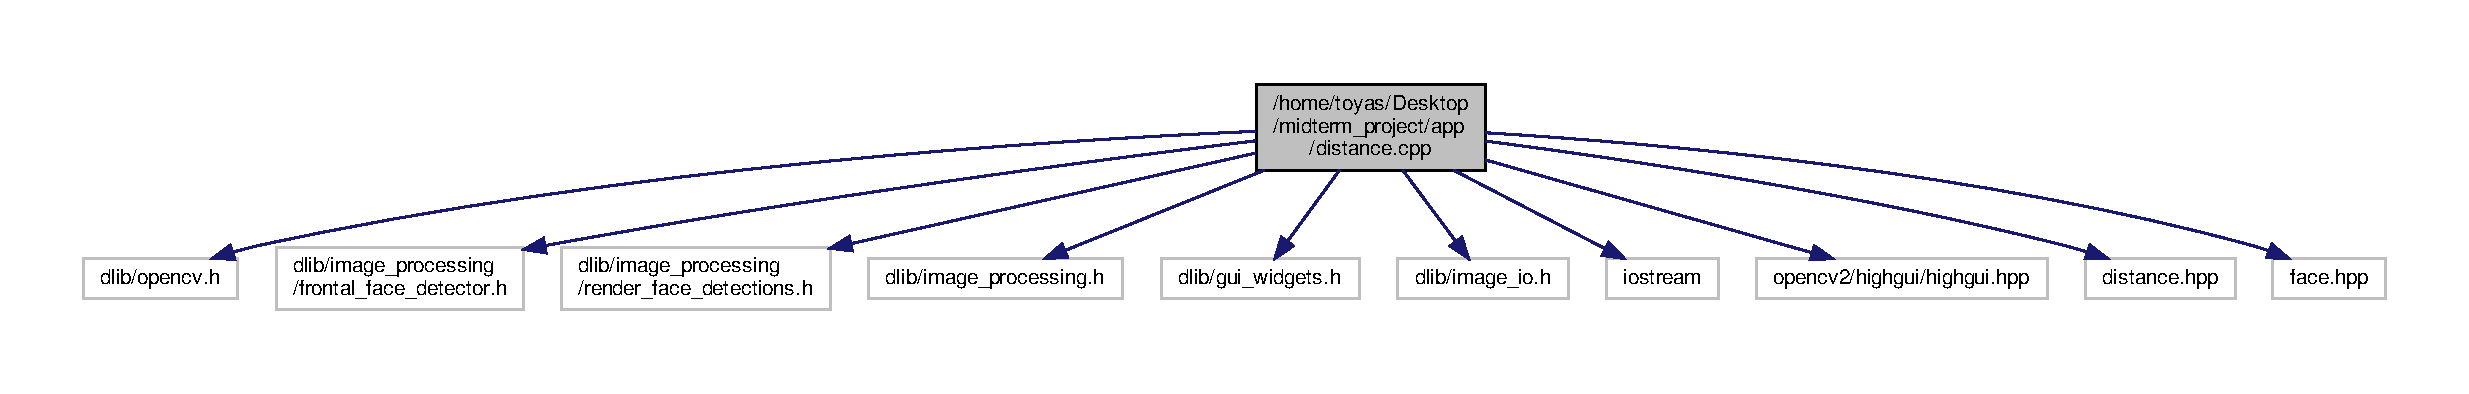
\includegraphics[width=350pt]{distance_8cpp__incl}
\end{center}
\end{figure}


\subsection{Detailed Description}
This is a class for depth perception module based on image from single camera. 

\begin{DoxyAuthor}{Author}
Toyas Dhake (Driver), Shivam Akhauri (Navigator) 
\end{DoxyAuthor}
\begin{DoxyDate}{Date}
11 October 2019 
\end{DoxyDate}
\begin{DoxyCopyright}{Copyright}
2019 Toyas Dhake, Shivam Akhauri 
\end{DoxyCopyright}

\hypertarget{face_8cpp}{}\section{/home/toyas/\+Desktop/midterm\+\_\+project/app/face.cpp File Reference}
\label{face_8cpp}\index{/home/toyas/\+Desktop/midterm\+\_\+project/app/face.\+cpp@{/home/toyas/\+Desktop/midterm\+\_\+project/app/face.\+cpp}}


This is a class to store porperties of face.  


{\ttfamily \#include $<$face.\+hpp$>$}\newline
Include dependency graph for face.\+cpp\+:
\nopagebreak
\begin{figure}[H]
\begin{center}
\leavevmode
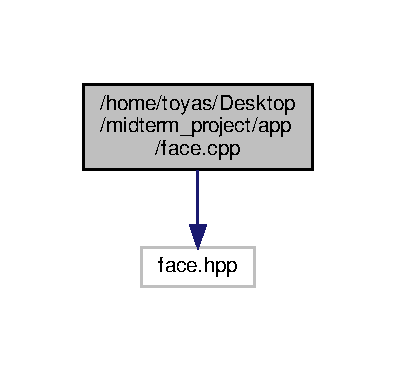
\includegraphics[width=190pt]{face_8cpp__incl}
\end{center}
\end{figure}


\subsection{Detailed Description}
This is a class to store porperties of face. 

\begin{DoxyAuthor}{Author}
Toyas Dhake (Driver), Shivam Akhauri (Navigator) 
\end{DoxyAuthor}
\begin{DoxyDate}{Date}
11 October 2019 
\end{DoxyDate}
\begin{DoxyCopyright}{Copyright}
2019 Toyas Dhake, Shivam Akhauri 
\end{DoxyCopyright}

\hypertarget{main_8cpp}{}\section{/home/toyas/\+Desktop/midterm\+\_\+project/app/main.cpp File Reference}
\label{main_8cpp}\index{/home/toyas/\+Desktop/midterm\+\_\+project/app/main.\+cpp@{/home/toyas/\+Desktop/midterm\+\_\+project/app/main.\+cpp}}


Main file for implementation of the Depth Perception project.  


{\ttfamily \#include $<$dlib/gui\+\_\+widgets.\+h$>$}\newline
{\ttfamily \#include $<$dlib/opencv.\+h$>$}\newline
{\ttfamily \#include $<$iostream$>$}\newline
{\ttfamily \#include $<$opencv2/highgui/highgui.\+hpp$>$}\newline
{\ttfamily \#include $<$distance.\+hpp$>$}\newline
{\ttfamily \#include $<$face.\+hpp$>$}\newline
Include dependency graph for main.\+cpp\+:
\nopagebreak
\begin{figure}[H]
\begin{center}
\leavevmode
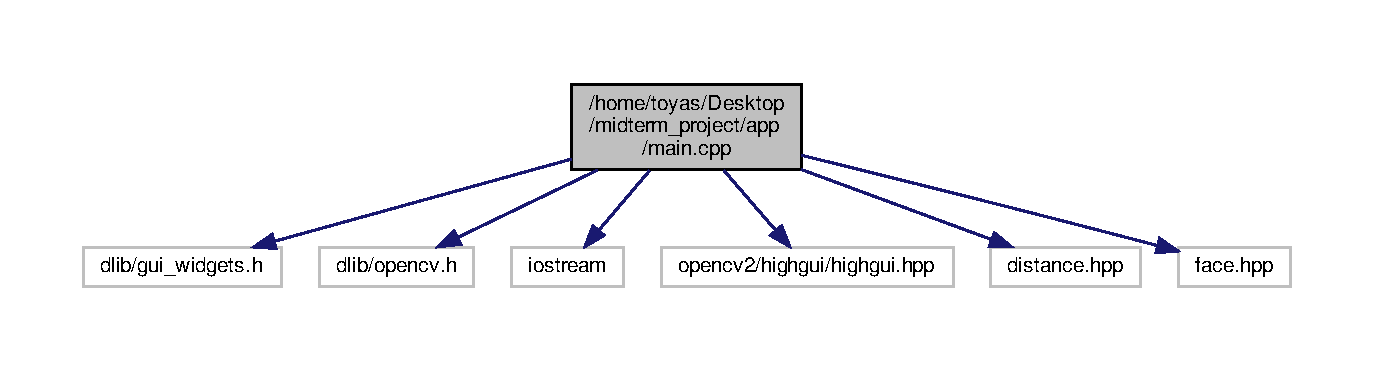
\includegraphics[width=350pt]{main_8cpp__incl}
\end{center}
\end{figure}
\subsection*{Functions}
\begin{DoxyCompactItemize}
\item 
int \hyperlink{main_8cpp_ae66f6b31b5ad750f1fe042a706a4e3d4}{main} ()
\end{DoxyCompactItemize}


\subsection{Detailed Description}
Main file for implementation of the Depth Perception project. 

\begin{DoxyAuthor}{Author}
Toyas Dhake (Driver), Shivam Akhauri (Navigator) 
\end{DoxyAuthor}
\begin{DoxyDate}{Date}
11 October 2019 
\end{DoxyDate}
\begin{DoxyCopyright}{Copyright}
2019 Toyas Dhake, Shivam Akhauri 
\end{DoxyCopyright}


\subsection{Function Documentation}
\mbox{\Hypertarget{main_8cpp_ae66f6b31b5ad750f1fe042a706a4e3d4}\label{main_8cpp_ae66f6b31b5ad750f1fe042a706a4e3d4}} 
\index{main.\+cpp@{main.\+cpp}!main@{main}}
\index{main@{main}!main.\+cpp@{main.\+cpp}}
\subsubsection{\texorpdfstring{main()}{main()}}
{\footnotesize\ttfamily int main (\begin{DoxyParamCaption}{ }\end{DoxyParamCaption})}

Loactions and distances of faces are stored in vector$<$\+Face$>$ can be either use to compute something else or add overlay on gui window.

There are 2 options for gui, opencv or dlib we are using dlib hence cv\+::\+Mat needs to be converted to dlib\+::cv\+\_\+image.

Definition at line 16 of file main.\+cpp.


%--- End generated contents ---

% Index
\backmatter
\newpage
\phantomsection
\clearemptydoublepage
\addcontentsline{toc}{chapter}{Index}
\printindex

\end{document}
